\documentclass[11pt]{beamer}
\usetheme{Madrid}
\usecolortheme{default}

\usepackage{amsmath}
\usepackage{amsfonts}
\usepackage{amssymb}
\usepackage{graphicx}
\usepackage{booktabs}
\usepackage{algorithm}
\usepackage{algorithmic}
\usepackage{tikz}
\usetikzlibrary{arrows,positioning}

\title{Item-Based Collaborative Filtering for Music Recommendation}
\subtitle{A Co-occurrence Matrix Approach}
\author{Group 4 \\ Tran Dang Khoa - 20280054 \\ Pham Tran Tan Phat - 20280070 \\ To Gia Bao - 22280006}
\date{\today}

\begin{document}

\frame{\titlepage}

\begin{frame}
\frametitle{Overview}
\tableofcontents
\end{frame}

\section{Problem Statement \& Dataset}

\begin{frame}
\frametitle{Music Recommendation Challenge}
\begin{block}{Objective}
Build a personalized music recommendation system using item-based collaborative filtering
\end{block}

\begin{columns}
\begin{column}{0.5\textwidth}
\textbf{Dataset Structure:}
\begin{itemize}
\item \textbf{user\_id}: Unique identifier for each user
\item \textbf{song\_id}: Unique identifier for each track
\item \textbf{listen\_count}: Number of times user played the song
\end{itemize}

\vspace{0.2cm}
\textbf{Data Characteristics:}
\begin{itemize}
\item No ratings, only interaction counts
\item Real-world music streaming data
\end{itemize}
\end{column}
\begin{column}{0.5\textwidth}
\textbf{Key Statistics:}
\begin{itemize}
\item Unique users: Large scale
\item Unique songs: Thousands
\item Train/Test split: 80/20
\item Data format: User-Item interaction matrix
\end{itemize}

\vspace{0.2cm}
\textbf{Data Quality:}
\begin{itemize}
\item No missing values
\item No duplicate entries
\end{itemize}
\end{column}
\end{columns}
\end{frame}

\begin{frame}
\frametitle{Dataset Details \& Preprocessing}
\begin{block}{Core Data Fields}
\begin{description}
\item[\textbf{user\_id}] User identifier - represents individual music listeners
\item[\textbf{song\_id}] Track identifier - represents individual songs in the catalog  
\item[\textbf{listen\_count}] Frequency of interaction - how many times user played the song
\end{description}
\end{block}

\begin{columns}
\begin{column}{0.5\textwidth}
\textbf{Why These Fields Matter:}
\begin{itemize}
\item \textbf{user\_id}: Enables personalization
\item \textbf{song\_id}: Items to recommend
\item \textbf{listen\_count}: Measures preference strength
\end{itemize}

\textbf{Data Insights:}
\begin{itemize}
\item Co-occurrence patterns reveal similarity
\end{itemize}
\end{column}
\begin{column}{0.5\textwidth}
\textbf{Preprocessing Steps:}
\begin{enumerate}
\item Load user-track interaction data
\item Filter users with ≥30 unique songs
\item Split into train/test (80/20)
\item Create user-item interaction matrix
\end{enumerate}

\textbf{Result:}
Clean, dense dataset focusing on engaged users with sufficient listening history
\end{column}
\end{columns}
\end{frame}

\section{Methodology}

\begin{frame}
\frametitle{Item Similarity Principle}
\begin{block}{Core Assumption}
\textit{"Songs listened to by similar users are likely to be similar to each other"}
\end{block}

\begin{center}
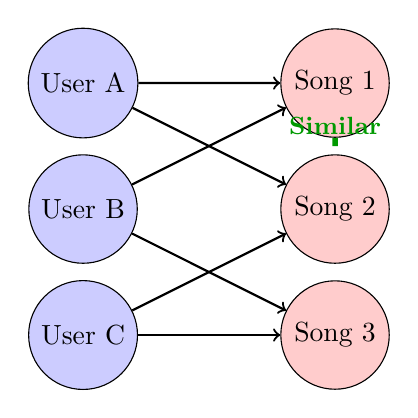
\begin{tikzpicture}[scale=0.8, node distance=1.5cm]
% Users
\node[circle, draw, fill=blue!20] (u1) at (0,2) {User A};
\node[circle, draw, fill=blue!20] (u2) at (0,0) {User B};
\node[circle, draw, fill=blue!20] (u3) at (0,-2) {User C};

% Songs
\node[circle, draw, fill=red!20] (s1) at (4,2) {Song 1};
\node[circle, draw, fill=red!20] (s2) at (4,0) {Song 2};
\node[circle, draw, fill=red!20] (s3) at (4,-2) {Song 3};

% Connections
\draw[->, thick] (u1) -- (s1);
\draw[->, thick] (u1) -- (s2);
\draw[->, thick] (u2) -- (s1);
\draw[->, thick] (u2) -- (s3);
\draw[->, thick] (u3) -- (s2);
\draw[->, thick] (u3) -- (s3);

% Similarity indication
\draw[dashed, thick, green!60!black, line width=2pt] (s1) -- (s2) node[midway, above, font=\small\bfseries] {Similar};
\end{tikzpicture}
\end{center}
\end{frame}

\begin{frame}
\frametitle{Algorithm Workflow}
\begin{algorithm}[H]
\caption{Item Similarity Recommender}
\begin{algorithmic}[1]
\STATE \textbf{Input:} User ID, Training Data
\STATE Get user's listening history: $S_u = \{s_1, s_2, ..., s_k\}$
\STATE Get all songs in system: $S_{all} = \{s_1, s_2, ..., s_n\}$
\STATE \textbf{For each} song pair $(s_i, s_j)$:
\STATE \quad Compute Jaccard similarity using co-occurrence
\STATE Build co-occurrence matrix $M_{k \times n}$
\STATE Compute weighted similarity scores
\STATE Rank songs by similarity scores
\STATE Filter out already-listened songs
\STATE \textbf{Return:} Top-10 recommendations
\end{algorithmic}
\end{algorithm}
\end{frame}

\section{Technical Implementation}

\begin{frame}
\frametitle{Co-occurrence Matrix Construction}
\begin{block}{Jaccard Similarity Formula}
\begin{equation}
J(s_i, s_j) = \frac{|U_{s_i} \cap U_{s_j}|}{|U_{s_i} \cup U_{s_j}|}
\end{equation}
where $U_{s_i}$ = set of users who listened to song $s_i$
\end{block}

\begin{columns}
\begin{column}{0.5\textwidth}
\textbf{Matrix Dimensions:} $k \times n$ 
\begin{itemize}
\item $k$ = user's songs, $n$ = total songs
\item Each cell = Jaccard similarity
\end{itemize}

\textbf{Quick Example:}
\small
Song A: \{User1, User2, User3\}, Song B: \{User2, User3, User4\} \\
Jaccard = $\frac{2}{4} = 0.5$ (50\% similar)
\textbf{Matrix:} $k \times n$ ($k$ = user's songs, $n$ = total)

\end{column}
\begin{column}{0.5\textwidth}


\begin{block}{Weighted Score Calculation}
\begin{equation}
Score(s_j) = \frac{1}{k} \sum_{i=1}^{k} J(s_i, s_j)
\end{equation}
\textbf{Example:} User \{Rock, Pop, Jazz\}, Blues similarities \{0.6, 0.2, 0.8\} \\
Score = $\frac{0.6+0.2+0.8}{3} = 0.53$
\end{block}
\end{column}
\end{columns}
\end{frame}



\begin{frame}[fragile]
\frametitle{Key Implementation Details}
\begin{block}{Data Preprocessing}
\begin{itemize}
\item Filter users with ≥30 unique songs (active users)
\item 80/20 train-test split
\end{itemize}
\end{block}

\begin{block}{Similarity Computation}
\small
\begin{verbatim}
# Jaccard Index calculation
users_intersection = users_i.intersection(users_j)
users_union = users_i.union(users_j)
similarity = len(users_intersection) / len(users_union)
\end{verbatim}
\end{block}

\begin{block}{Recommendation Generation}
\begin{itemize}
\item Compute average similarity across all user's songs
\item Sort by similarity score (descending)
\item Filter out previously listened songs
\item Return top-10 recommendations
\end{itemize}
\end{block}
\end{frame}

\section{Evaluation \& Results}

\begin{frame}
\frametitle{Evaluation Methodology}
\begin{block}{Metrics Used}
\begin{itemize}
\item \textbf{Precision@K}: $\frac{\text{Relevant items in top-K}}{\text{K}}$
\item \textbf{Recall@K}: $\frac{\text{Relevant items in top-K}}{\text{Total relevant items}}$
\item Evaluated for K = 1, 2, ..., 10
\end{itemize}
\end{block}

\begin{block}{Experimental Setup}
\begin{itemize}
\item User sample: 5\% of test users
\item Test data: 1000 records subset
\item Recommendations: Top-10 per user
\item Ground truth: User's actual listening in test set
\end{itemize}
\end{block}

\textbf{Precision-Recall Curve:} Shows trade-off between precision and recall across different K values
\end{frame}

\begin{frame}
\frametitle{Results: Impact of User Filtering}
\begin{columns}
\begin{column}{0.5\textwidth}
\textbf{Before Filtering (All Users):}
\begin{itemize}
\item \textbf{Precision@10}: Up to 20\%
\item \textbf{Recall@10}: Up to 12.5\%
\item Curve position: Center to upper-left
\item Includes casual users (1-5 songs)
\end{itemize}

\vspace{0.3cm}
\textbf{After Filtering (≥30 songs):}
\begin{itemize}
\item \textbf{Precision@10}: 7.5-10\%
\item \textbf{Recall@10}: ~2.5\%
\item Curve position: Lower-left corner
\item Only active, engaged users
\end{itemize}
\end{column}
\begin{column}{0.5\textwidth}
\begin{center}
\textbf{Performance Comparison:}
\small
\begin{tabular}{|l|c|c|}
\hline
\textbf{Metric} & \textbf{Before} & \textbf{After} \\
\hline
Max Precision & 20\% & 10\% \\
Max Recall & 12.5\% & 2.5\% \\
User Quality & Mixed & High \\
Realism & Low & High \\
\hline
\end{tabular}

\vspace{0.3cm}
\textbf{Why the Drop?}
\begin{itemize}
\item Casual users = easy predictions
\item Active users = complex preferences
\item Filtered results more realistic
\end{itemize}
\end{center}
\end{column}
\end{columns}
\end{frame}

\begin{frame}
\frametitle{Precision-Recall Curves Comparison}
\begin{columns}
\begin{column}{0.5\textwidth}
\begin{center}
\textbf{Before Filtering}
\includegraphics[width=\textwidth]{not-filtered-plot.png}
\small

\end{center}
\end{column}
\begin{column}{0.5\textwidth}
\begin{center}
\textbf{After Filtering (≥30 songs)}
\includegraphics[width=\textwidth]{filtered-plot.png}
\small

\end{center}
\end{column}
\end{columns}

\begin{block}{Key Insight}
\textbf{Performance drop is expected and desirable} - it indicates proper evaluation methodology focusing on meaningful user segments
\end{block}
\end{frame}

\begin{frame}
\frametitle{Why User Filtering Improves Evaluation Quality}
\begin{block}{The "Easy Prediction" Problem}
\textbf{Casual Users (1-5 songs):} Small test sets → Artificially high precision/recall
\end{block}

\begin{columns}
\begin{column}{0.5\textwidth}
\textbf{Mathematical Example:}
\small
\begin{align}
\text{Casual User:} \nonumber \\
\text{Test songs} &= 1 \nonumber \\
\text{Correct predictions} &= 1 \nonumber \\
\text{Precision} &= \frac{1}{1} = 100\% \nonumber
\end{align}

\begin{align}
\text{Active User:} \nonumber \\
\text{Test songs} &= 8 \nonumber \\
\text{Correct predictions} &= 1 \nonumber \\
\text{Precision} &= \frac{1}{8} = 12.5\% \nonumber
\end{align}
\end{column}
\begin{column}{0.5\textwidth}
\textbf{Business Relevance:}
\begin{itemize}
\item \textbf{Active users}: Generate revenue, stay engaged
\item \textbf{Casual users}: May not return, limited value
\item \textbf{Filtering focus}: Real users
\item \textbf{Realistic metrics}: True system performance
\end{itemize}

\textbf{Industry Standard:}
Music platforms evaluate on users with sufficient listening history (≥20-50 songs)
\end{column}
\end{columns}
\end{frame}

\section{System in Action}

\begin{frame}
\frametitle{User's Listening History}
\begin{block}{Step 1: Input Data}
Display the songs that the selected user has already listened to in the training data
\end{block}

\begin{center}
\includegraphics[width=0.8\textwidth]{songs-of-user.png}
\end{center}

\begin{block}{Analysis}
\begin{itemize}
\item Shows user's historical music preferences
\item Forms the basis for similarity calculations
\item Used to find similar songs for recommendations
\end{itemize}
\end{block}
\end{frame}

\begin{frame}
\frametitle{Generated Recommendations}
\begin{block}{Step 2: System Output}
Top 10 personalized song recommendations with similarity scores and rankings
\end{block}

\begin{center}
\includegraphics[width=0.8\textwidth]{results.png}
\end{center}

\begin{block}{Key Features}
\begin{itemize}
\item Ranked by similarity score (highest first)
\item Excludes songs user has already heard
\item Provides interpretable confidence scores
\end{itemize}
\end{block}
\end{frame}

\begin{frame}
\frametitle{System Output Interpretation}
\begin{block}{Understanding the Results}
\begin{itemize}
\item \textbf{User ID}: Identifies the target user for recommendations
\item \textbf{Song ID}: Unique identifier for each recommended track
\item \textbf{Score}: Weighted similarity score (0-1 scale)
\item \textbf{Rank}: Recommendation priority (1 = highest)
\end{itemize}
\end{block}

\begin{columns}
\begin{column}{0.5\textwidth}
\textbf{Key Observations:}
\begin{itemize}
\item Recommendations exclude already-listened songs
\item Scores reflect similarity to user's taste profile
\item Higher scores indicate stronger recommendations
\item System provides explainable results
\end{itemize}
\end{column}
\begin{column}{0.5\textwidth}
\textbf{Practical Benefits:}
\begin{itemize}
\item \textbf{Personalized}: Based on individual listening history
\item \textbf{Relevant}: Similar to user's existing preferences
\item \textbf{Ranked}: Clear priority ordering
\item \textbf{Interpretable}: Scores show confidence level
\end{itemize}
\end{column}
\end{columns}

\begin{block}{Real-World Application}
This demonstrates how the system works in practice - taking a user's listening history and generating meaningful, personalized music recommendations that align with their taste profile.
\end{block}
\end{frame}

\section{Advantages \& Limitations}

\begin{frame}
\frametitle{Strengths \& Weaknesses}
\begin{columns}
\begin{column}{0.5\textwidth}
\textbf{✅ Advantages:}
\begin{itemize}
\item \textbf{Personalized}: Based on actual user behavior
\item \textbf{Explainable}: "Because you liked X, try Y"
\item \textbf{No content needed}: Only interaction data
\item \textbf{Domain agnostic}: Works across different domains
\item \textbf{Quality recommendations}: Similar items tend to be relevant
\end{itemize}
\end{column}
\begin{column}{0.5\textwidth}
\textbf{❌ Limitations:}
\begin{itemize}
\item \textbf{Cold start}: Can't recommend to new users
\item \textbf{Sparsity}: Matrix mostly zeros
\item \textbf{Scalability}: Expensive computation for large datasets
\item \textbf{Echo chamber}: May lack diversity
\item \textbf{Popular bias}: Tends to recommend popular items
\end{itemize}
\end{column}
\end{columns}

\begin{block}{Best Use Cases}
Music streaming, e-commerce, movie recommendations where user-item interactions are abundant
\end{block}
\end{frame}

\section{Conclusion}

\begin{frame}
\frametitle{Summary \& Future Work}
\begin{block}{Key Achievements}
\begin{itemize}
\item Successfully implemented item-based collaborative filtering
\item \textbf{Demonstrated importance of user filtering} for realistic evaluation
\item Achieved meaningful precision-recall performance (7-10\% precision for active users)
\item \textbf{Revealed evaluation bias} in unfiltered data (artificially high metrics)
\item Created scalable, interpretable recommendation system
\end{itemize}
\end{block}

\begin{block}{Critical Insights}
\begin{itemize}
\item \textbf{User filtering is essential}: Prevents inflated metrics from casual users
\item \textbf{Performance drop is good}: Indicates realistic, challenging evaluation
\item \textbf{Focus on engaged users}: More business-relevant metrics
\end{itemize}
\end{block}

\begin{block}{Future Improvements}
\begin{itemize}
\item \textbf{Hybrid approach}: Combine with content-based filtering
\item \textbf{Deep learning}: Neural collaborative filtering
\item \textbf{Temporal dynamics}: Account for changing preferences
\item \textbf{Diversity optimization}: Reduce echo chamber effect
\end{itemize}
\end{block}
\end{frame}

\begin{center}
\Large{\textbf{Thank you for your attention!}}
\end{center}
\end{frame}

\end{document}
